%-----------------------------------------------------------------------------------------------
%		\COMPdataPartManagement{} Design
%-----------------------------------------------------------------------------------------------

\section{\COMPdataPartManagement{} Design}
\label{sec:COMPdataBlockManagementDesign}

In this section, the design of the component \COMPdataPartManagement{} is described. Basic task of the component is to implement the actual generic parsing of data of a supported data format in a well-performing, yet flexible and extensible way.
% =======================================================================================================
\subsection{Basic Concept for Reading}%
\label{sec:BasicConceptforReading}%

In section \SectionLink{sec:RepresentingaDataFormat}, we discussed the approach that a data format is described in terms of a \emph{data format specification}, which basically is a description of how data is represented as a chunk of bytes in the data format. It breaks up such a chunk into different types of so-called data blocks that form a well-defined hierarchy (see \SectionLink{sec:TheContainerMetamodel}). Given such a specification and data block hierarchy, we define the following design decisions:

%%%% DD --> %%%%
\DD{dd:601}
{% Title
Data block instance classes defined in \COMPdataPartManagement{}
}
{% Short description
The instances for the different data block types are represented as Java classes in the \COMPdataPartManagement{} component which use the same names as in figure \ref{fig:II_GeneralModel}.
}
{% Rationale
As chunks of bytes are structured according to the metamodel and the data format specification describes them as such, it is quite clear the have to be instance of corresponding classes during parsing. These instances are also returned to the user and provide a clear, better-to-understand view on the data. Btw., having a metamodel but not transforming it into a class model seems to be quite nonsense.
}
{% Disadvantages
No disadvantages known.
}
%%%% <-- DD %%%%

%%%% DD --> %%%%
\DD{dd:602}
{% Title
Specification-driven Read Approach
}
{% Short description
Reading is heavily based on the description of the data format in its data format specification. The descriptions of lengths and types are used as basic assumption for parsing, especially magic keys for first identification.
}
{% Rationale
It is quite clear that otherwise, the data format specification would be quite useless and we would implement some data-format-specific and thus non-generic code again.
}
{% Disadvantages
Is it flexible enough? If we stick to a stiff specification, how to ensure that it is flexible enough for different data formats?
}
%%%% <-- DD %%%%

%%%% DD --> %%%%
\DD{dd:603}
{% Title
Reading and writing with \COMPmedia{}
}
{% Short description
Reading and writing is done using \COMPmedia{}, including use of its caching features.
}
{% Rationale
Again this is very clear.
}
{% Disadvantages
No disadvantages known.
}
%%%% <-- DD %%%%

Given these basic design decisions, we are ready to sketch a rough draft of how reading basically works. We first summarize the very fundamentals that we know this far:
\begin{itemize}
\item Data is represented as linear chunks of bytes whose structure is defined by the data format specification
\item The top-level data blocks for reading are containers
\item It is not clear which data format we have in front of us
\item A data block might get large, as we use long as data type (see \DesLink{dd:417})
\end{itemize}

Given the first two observations, we define the following:

%%%% DD --> %%%%
\DD{dd:604}
{% Title
Iterator approach for reading
}
{% Short description
  \LibName{} provides an iterator pattern for iterating top-level containers.
}
{% Rationale
As the basic structure of a chunk of data format bytes consists of linear disjoint containers and we need to do forward-reading, an iterator is a quite natural choice. Lists or other collection data types would be insufficient, because they would suggest that there is a finite number of containers. Iterators are a good fit for streaming, allowing virtually ``unlimited'' streams of containers.
}
{% Disadvantages
No disadvantages known.
}
%%%% <-- DD %%%%

Now we can define the basis approach of forward reading, i.e. what is done if we read a top-level container? Of course, first it is not clear which data format we have - identification is necessary, already introduced in \SectionLink{sec:MagicKeys}. Second, it might happen anytime that we hit end of medium, either expectedly or unexpectedly. The basic flow is defined in the following design decision and shown in figure \ref{fig:III_ForwardReading}.

\begin{figure}[htbp]
  \centering
  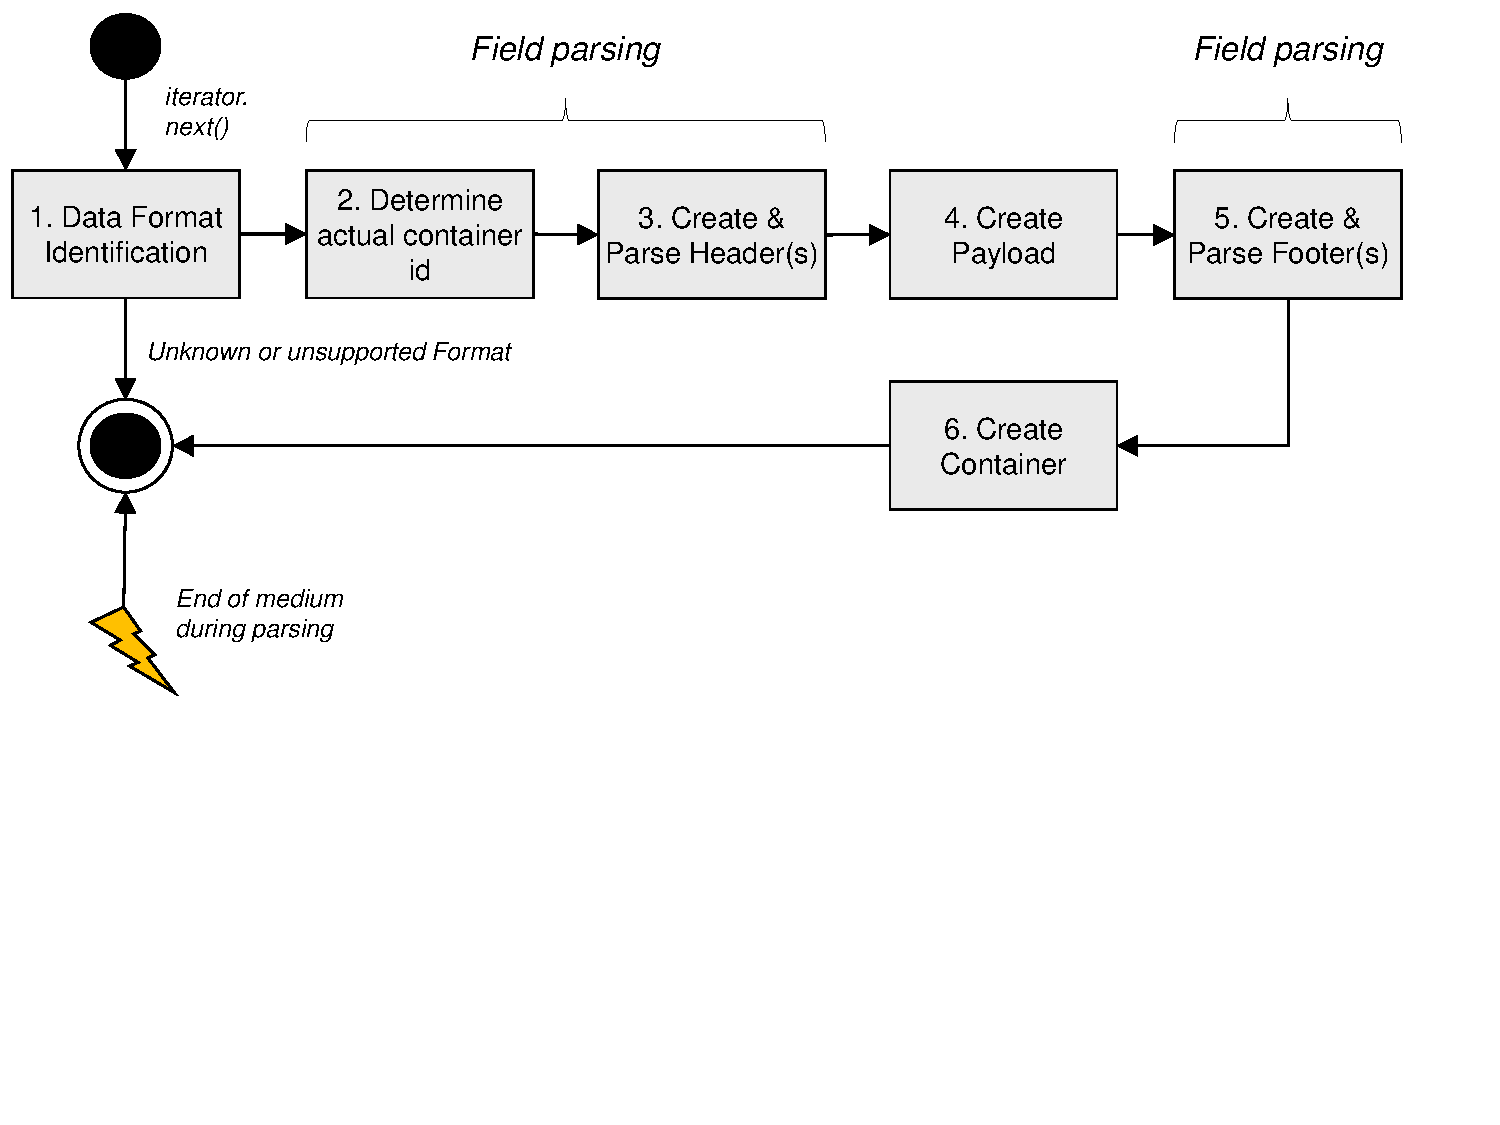
\includegraphics[width=1.0\linewidth]{figures/III_ForwardReading.pdf}
  \caption{Steps for reading data forward}
  \label{fig:III_ForwardReading}
\end{figure}

%%%% DD --> %%%%
\DD{dd:605}
{% Title
Steps of forward reading of top-level containers
}
{% Short description
  Forward reading of a single top-level container works as follows - whenever \texttt{next()} on the iterator is called to read the first or next container:
  \begin{enumerate}
  \item First, we do data format identification, i.e. finding out whether the data chunk ahead belongs to a data format the library supports - see \SectionLink{sec:MagicKeys} for details. If we cannot identify the data format, the process stops here with an exception.
  \item After identifying the data format, we need to identify which concrete container we have, i.e. determining its actual id at runtime; this is necessary for data formats supporting generic containers which is most of the container data formats out there. 
  \item Then, as we forward-read, the headers of the container are parsed, which means understanding their content. This includes determining if there are other headers or footers, and also the length of the container's payload.
  \item After heaving determined the payload length, the payload object itself is created. 
  \item Then, if there are any footers, they are at least created and ready to be parsed.
  \item Finally, the container is created which consists of the previously created headers, footers and payload
  \end{enumerate}
  It might happen that during this process, an expected or unexpected end of medium occurs. Expected it can only be during data format identification, in all other cases there seems to be a corruption in the data or parallel changes, as the parsing metadata indicates a size which is not matching reality.

  During steps 2, 3 and 5, fields need to be parsed which is a special discipline discussed later.
}
{% Rationale
The process is aligned at the structure of a container and typical for forward reading.
}
{% Disadvantages
No disadvantages known.
}
%%%% <-- DD %%%%

% =======================================================================================================
\subsection{Buffering, Caching and Lazy Reading}%
\label{sec:ReadingSteps}%

\COMPdataPartManagement{} uses the features of \COMPmedia{} for caching as described in \SectionLink{sec:PerfMedia}. These features are also used for buffering, i.e.
%%%% DD --> %%%%
\DD{dd:606}
{% Title
Headers are buffered during forward reading
}
{% Short description
For static headers, they are buffered as a whole by first caching all bytes the header is made of; for dynamic-length headers, headers are buffered according to their known minimum length. Any upcoming fields are read using \COMPmedia{}'s \texttt{getData} and thus either use the buffered data or fetch it from the medium.
}
{% Rationale
Reading byte by byte or field by field would be nonsense from performance point of view
}
{% Disadvantages
No disadvantages known.
}
%%%% <-- DD %%%%

During data format identification, the library might need to ``try'' multiple different magic keys to see what data format is ahead. This process is optimized as follows:
%%%% DD --> %%%%
\DD{dd:606a}
{% Title
Use longest header size for initial buffering
}
{% Short description
The buffering in \DesLink{dd:606} first calculates a minimum suitable size to read by obtaining the minimum sizes of all headers of all supported data format's top-level containers. It chooses the longest such size for its purpose. Thus, clearly, end of medium might be reached if a long header is read first while the actual data format has a short header and the medium ands early. Such an end of medium condition is not an error but simply rules out some candidate data formats.
}
{% Rationale
Otherwise we would probably do some very inefficient piece-wise reading during data format identification
}
{% Disadvantes
No disadvantages known
}
%%%% <-- DD %%%%

A very basic mechanism of container data formats is that they allow seeking and skipping based on containers, that means the decoders might just need to check a container header to find out if they are interested in the data it contains, and if not simply go on reading with the follow-up container. For this, most if not all data formats specify the size of the container in its header or footer. To fully support this, we define some kind of lazyness as follows:

%%%% DD --> %%%%
\DD{dd:607}
{% Title
Lazy payload
}
{% Short description
Any field-based or container-based payload is lazy by default, i.e. its bytes are first read only when explicitly requested by the user. A sole exception is in place for stream-based media (see upcoming design decision). 
}
{% Rationale
This way, we do not read unnecessary data the user might never look at, especially allowing to skip over large containers without risking out of memory and long read times, just perfectly meeting requirement \SectionLink{sec:REQ009LesenSchreibenGrosse}.
}
{% Disadvantes
No disadvantages known
}
%%%% <-- DD %%%%

As streams are non-random-access media, the question arises what we do with the bytes of a stream. It is no good idea to skip the payload byte here - what if the user wants to closely look at them? There is no other choice than to still cache them. The same is true for rather ``exotic'' formats such as Lyrics3v2 where the payload size is not contained in a header, but only in the footer.

%%%% DD --> %%%%
\DD{dd:608}
{% Title
Fully cache payload for stream-based media and formats without size field
}
{% Short description
  For stream-based media, the whole payload data must be fully read to at least have a chance that the user can look at it later. It might happen that the maximum cache size is exceeded in which case the first bytes of the payload might fall out of the cache.

For formats not having a static payload size and not having a size indicator in its header, the payload must be fully read in entirety to know its size. This also leads to potentially filling up the cache. 
}
{% Rationale
  There is no other way for streams than grabbing the bytes when looking at them - streams are just one time read.

  For the special case of formats not having a payload size in their header, see \DesLink{dd:529d}.
}
{% Disadvantes
No disadvantages known
}
%%%% <-- DD %%%%

% =======================================================================================================
\subsection{Field Parsing}%
\label{sec:FieldParsing}%

Field parsing is the most complex part of reading data format bytes. It requires answers to following questions:
\begin{itemize}
\item How to determine the size of the field?
\item How to determine the number of occurrences of a field, especially the case of optional fields?
\item Which byte order (for numeric fields) and character encoding (for string or enumerated fields) needs to be used when?
\item How to convert the binary field value to an interpreted one?
\item How to use caching during field parsing?
\end{itemize}

% -------------------------------------------------------------------------------------------------------
\subsubsection{Terminated Fields}%
\label{sec:TerminatedFields}%

Terminated fields are those fields with a dynamic length that is not given by the value of another field, but these fields are delimited by a sequence of termination bytes or characters. 

Terminated fields are worst-case for parsing: First of all you never know when it ends, and second you have to deal with strings which brings different encodings into play.

Let's deal with the first problem, the unknown length. Of course, in the ``usual'' case a terminated field is still a field and thus relatively small. We will only rarely encounter terminated fields longer than several KB. In order to be fully generic, one needs to deal with the worst case of fields having up to \texttt{Long.MAX\_VALUE-1} as size. Having said this, also block-wise reading is required as we do not want to risk out-of-memory conditions by soaking too much bytes into memory. One could come up with the idea of using some upper bounds for reading data, i.e.:
\begin{itemize}
\item \textbf{Case 1:} The current total medium size as well as the exact size of a parent of the field is known - E.g. for ID3v23 text frames, the frame size and thus payload size is known, but there is a terminated text payload field; for file and byte array media, the medium length is also known.
\item \textbf{Case 2:} The current total medium size is unknown, yet the exact size of a parent of the field is known - Take an ID3v23 text frame on an input stream medium as an example.
\item \textbf{Case 3:} The current total medium size is known, but the exact size of a parent of the field is unknown - Take an APEv2 item header on a file or byte array medium as an example. Here, the item key is terminated, and the size of the parent header is unknown as it is only determined by the sum of the field sizes and not - in addition - by any size indicators.
\item \textbf{Case 4:} Neither current total medium size nor the exact size of a parent of the field is known - So APEv2 item header on an input stream medium is an example.
\end{itemize}

%%%% DD --> %%%%
\DD{dd:650a}
{% Title
Block-wise reading for finding field termination
}
{% Short description
Block-wise reading is necessary in order to find field termination. According to \DesLink{dd:438}, we do not read more than the configured maximum read-write block size in bytes from the medium at once. Actually, we \emph{always} read the configured maximum read-write block size and do not take into consideration any additionally known upper bounds such as the remaining parent byte count or remaining medium length (if available). If an end of medium is encountered during reading a block of data, we scan for the termination within the actually read bytes. Otherwise the next block is read for scanning for termination bytes and so on. However, we can at least take into account any available bounds for finding out if we need to search further or we can skip the process: If the already read byte count is bigger than the remaining parent byte count, we should skip as a data corruption might be present.
}
{% Rationale
Block-wise reading avoids out-of-memory conditions and is a compromise between reading too much and reading too few bytes at once. Of course this compromise comes with the cost of added complexity. We mitigate this complexity by not coming up with further ``optimizations'' such as only reading up to a known upper bound like the medium end or parent end. In the end, both might not be known, especially in case 4, thus anyway we have to do a ``blind'' reading in this case.
}
{% Disadvantes
Added complexity, but in conformance with \DesLink{dd:438}. The complexity is adressed as specified in the rationale.
}
%%%% <-- DD %%%%

Regarding strings and their encoding: First of all, we remember that only string and string list fields can be terminated and thus it is fine to talk about \emph{termination characters} instead of termination bytes (see \DesLink{dd:531} and \DesLink{dd:532}). How should we parse terminated fields to detect the termination character? We could do it either:
\begin{enumerate}
\item by converting the character to a byte sequence and then searching the termination
\item by converting the bytes to a string and then trying to find the termination character or
\end{enumerate}

Both approaches have their serious drawbacks. \textbf{Approach (1)} requires us to know where a character starts and ends such that we can correctly match termination bytes only at character borders. For instance UTF-16 encodes all characters always as two bytes. It would be wrong to try to detect termination bytes at odd offsets. Instead we have to ensure to search for them only at even offsets.

\textbf{Approach (2)} suffers from a similar problem that there is no nice way to handle block-wise split strings: If we read block-wise, it might be that a single character spanning multiple bytes is just torn apart at a block border. E.g. UTF-8 is a variable length encoding where - depending on the first byte - the total number of bytes of a character is given. If a converter from byte to string encounters a torn apart character at the end of the byte sequence, it might fail with some kind of decoding runtime error, so we have to handle this separately. However, Java's \texttt{CharsetDecoder} seems just about right for this task. ID3v2.4 supports UTF-16LE, UTF-16BE, ISO-8859-1 as well as UTF-8 so we have to handle such cases.

We define:
%%%% DD --> %%%%
\DD{dd:650}
{% Title
Character-based termination detection
}
{% Short description
We use character-based termination detection (approach 2) for finding termination characters and do not use termination-byte-based detection (approach 1)
}
{% Rationale
This is possible due to the fact that only string and string list fields can be terminated (see \DesLink{dd:531} and \DesLink{dd:532}). Approach 1 seems even harder as we need to re-implement parsing of strange encodings while approach 2 at least provides an out-of-the box solution in the form of  \texttt{CharsetDecoder}.
}
{% Disadvantes
No disadvantages known
}
%%%% <-- DD %%%%

No we can summarize the process of finding termination of a field:
%%%% DD --> %%%%
\DD{dd:651}
{% Title
Determining the end of a terminated field
}
{% Short description
  As input for the algorithm, we get the current medium offset, the character encoding of the bytes as well as the termination character to find and the maximum read-write block size. The steps are as follows:
  \begin{enumerate}
  \item Read $N:=$ read-write block size bytes from the medium at the current offset
  \item If end of medium occurs, take the actually read bytes and mark the algorithm for termination as no further input is available
  \item Search the input buffer for the termination character by actually decoding bytes according to the character encoding using \texttt{CharsetDecoder}
  \item If there should be a character overlapping a block border, use the facilities of \texttt{CharsetDecoder} to overcome the situation
  \item If a termination character is found, mark the algorithm for termination
  \item Otherwise:
    \begin{enumerate}
    \item If the remaining parent byte count is known and the already read byte count is bigger than this value, mark the algorithm for termination 
    \item Otherwise increment the current medium offset by the maximum read-write block size and goto step 1
    \end{enumerate}
  \end{enumerate}
}
{% Rationale
This process is efficient in terms of avoiding unknown steps and using only sparse memory. It is as simple as it can get without risking incorrectness.
}
{% Disadvantes
No disadvantages known
}
%%%% <-- DD %%%%

% =======================================================================================================
\subsection{Backward Reading}%
\label{sec:BackwardReading}%

% =======================================================================================================
\subsection{API Design}%
\label{sec:APIDesign}%












%###############################################################################################
%###############################################################################################
%
%		File end
%
%###############################################################################################
%###############################################################################################